
\section{Accelerators and Detectors: Basic Principles}
%%\begin{itemize}
%%    \item from the start; Magnetic rigidity(?)
%%    \item acceleration
%%    \item magnetic focussing, FODO, dipole, quadropole
%%    \item detector basics, (relevant) detector types, basic of bethe bloch
%%    \item luminosity calculations, bunch and crossings
%%    \item cross section
%%    \item Limiting factors
%%\end{itemize}


\section{The Large Hadron Collider}
The Large Hadron Collider (LHC) is a modern proton-proton synchrotron located at the CERN complex, outside of Meyrin, Switzerland. At a circumference of approximately 27km the LHC is currently the largest particle accelerator on the planet, and similarly produces the highest centre-of-mass energies for pp collisions, reaching $\sqrt{s}=13\text{TeV}$. The LHC was constructed from 1998-2008 in the tunnel previously occupied by the Large Electron-Positron Collider (LEP). It extends from from the CERN site, across the French border towards the Jura Mountains and round returning through Geneve and Meyrin. It is positioned on a plane inclined at $1.41\%$ between 45-175 metres underground, a measure to protect both the experimental recordings from a large fraction of cosmic ray interference and the surface from any hazardous emissions from either the particle collisions or the synchrotron radiation.

The LHC is supported by a number of smaller accelerator systems designed to provide proton bunches of the correct spacing and energy, these are visible in figure \ref{fig:accel_complex}. The acceleration process begins with the injection of Hydrogen anions ($\text{H}^{-}$) into LINAC\footnote{This was LINAC 2 until 2020, reaching $50\text{MeV}$. During Long Shutdown 2 (LS2) this was obsolesced by LINAC 4}, which provides an acceleration to energies of $160\text{MeV}$ before the beam is passed on the Proton Synchrotron Booster (PSB)\footnote{\href{https://cds.cern.ch/journal/CERNBulletin/2016/32/News\%20Articles/2201549?ln=en}{idk psb}}. This continuous beam from LINAC is stripped of electrons and split consecutively amongst the four PSB rings, accelerated to $1.4\text{GeV}$, and injected into the Proton Synchrotron (PS). PS produces bunches spaced by $25\text{ns}$, accelerates these to $25\text{GeV}$, and passes them over to the Super Proton Synchrotron (SPS) for the final energy increase up to $450\text{GeV}$.


% https://physics.stackexchange.com/questions/474122/how-is-a-proton-beam-separated-into-bunches-in-a-particle-accelerator
%%https://cds.cern.ch/record/446600/
%% "we must make sure that the particle always sees an accelerating voltage at the gap, so the RF frequency must always be an integer multiple (h) of the revolution frequency."
%% https://www.lhc-closer.es/taking_a_closer_look_at_lhc/0.buckets_and_bunches
%% https://home.cern/science/accelerators


%%SPS, LHC, fills reaching an energy of 13.6TeV, 6.8TeV per beam
%%
%%Accelerated by RF Cavities oscillating at 400MHz
%%
%%
%%The LHC 'ring'
%%
%%Dual-core beampipe, common cryostat
%%1232 dipoles, Niobium-titanite construction, ~8.3T at 1.9K
%%474 Quadropoles
%%
%%The Focussing process is performed 



%Points to make
%\begin{itemize}
%    \item precise location
%    \item geometry, straight and curved sections 
%    \item points and active experiments
%    \item full accelerator complex rundown, energies, etc
%    \item run details peak luminosities
%    \item upgrades and futures
%    \item effects of high energies, pileup, etc
%    \item bunch details, bunch grouping, injection etc
%    \item cosmics and radiation protection
%\end{itemize}

\begin{figure}[!h]
    \centering
    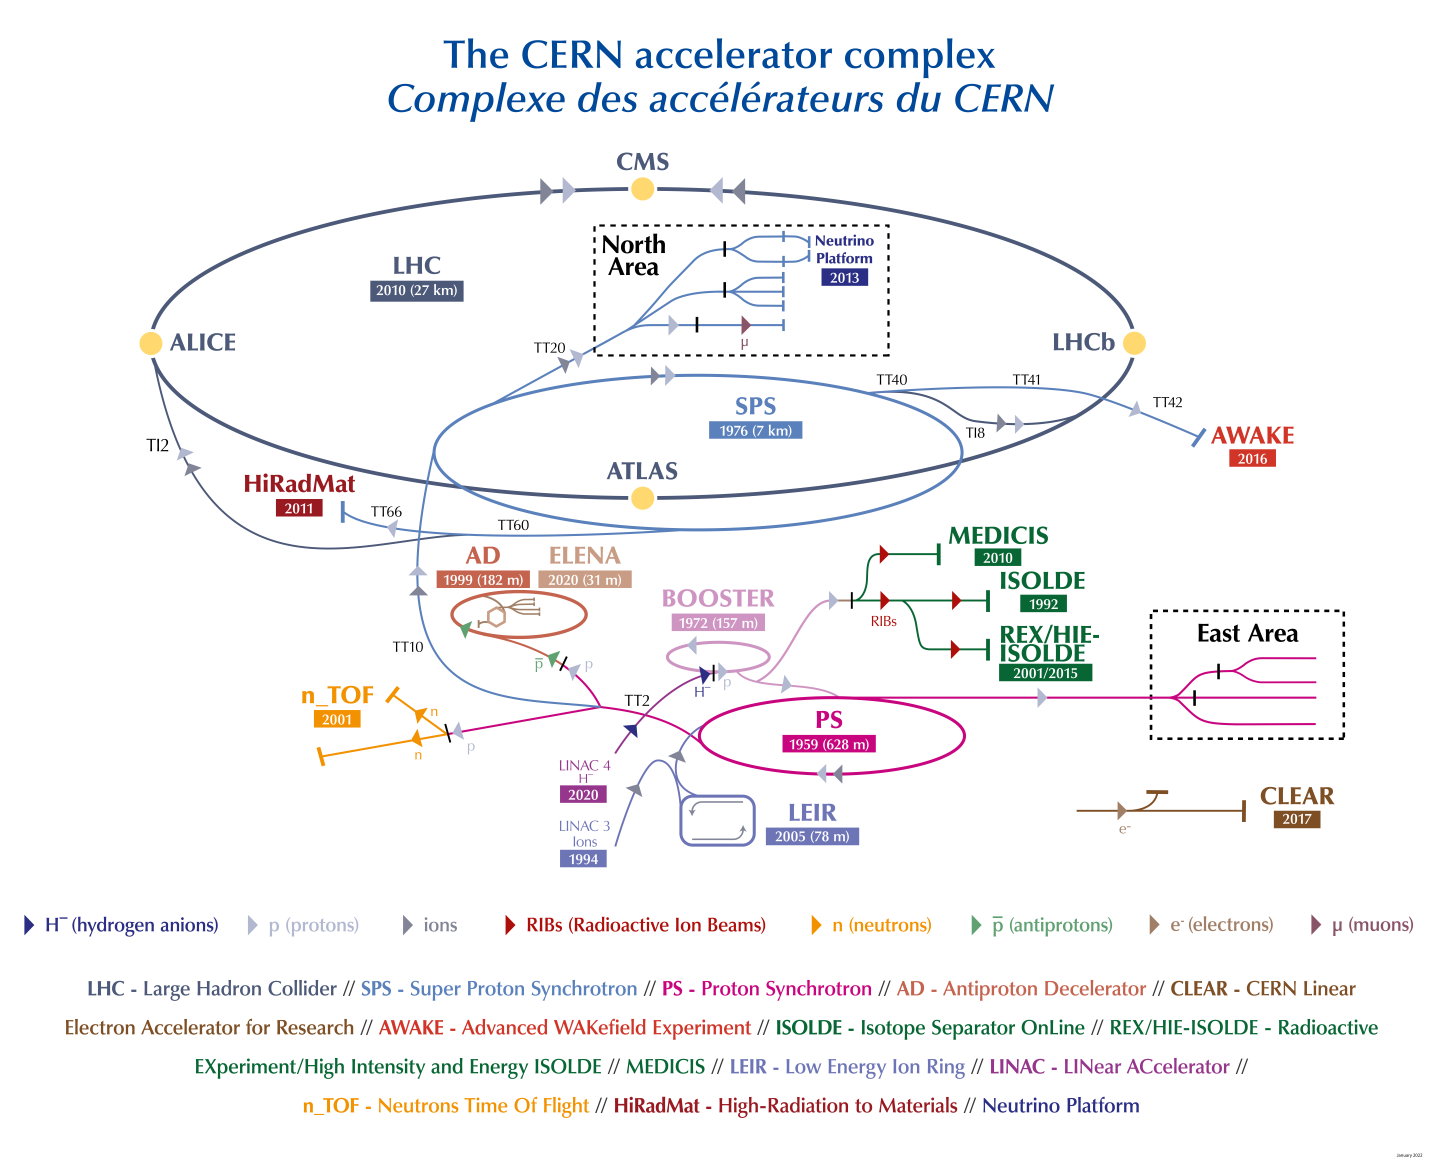
\includegraphics[]{figures/lhc_and_atlas/CCC-v2022.png}
    \caption{CERN Accelerator Complex schematic \cite{Lopienska:2800984}. }
    \label{fig:accel_complex}
\end{figure}




\section{The ATLAS Detector}
\subsection{Overview}
The ATLAS Detector[CITATION] as a general-purpose detector with cylindrical geometry and a forwards-backwards symmetry. It has nearly complete coverage, approaching $4\pi$, in solid angle around the interaction point (IP) which is located centrally within the detector layout.
%%\begin{itemize}
%%    \item Basic detector details.
%%    \item Some collaboration details.
%%    \item Location and control room.
%%    \item Sides.
%%    \item Support infrastructure.
%%\end{itemize}


\subsection{Coordinate system and common variables}
%%\begin{itemize}
%%    \item Rapidity
%%    \item Pseudorapidity
%%    \item Azimuthal angle
%%    \item eta-phi space
%%    \item impact parameters
%%    \item Other varibles required for track definition
%%    \item Common kinematic and analysis variables
%%\end{itemize}

%%\subsection{Inner Detector}
%%\begin{itemize}
%%    \item IBL
%%    \item SCT
%%    \item Pixel
%%    \item Transition Radiation Tracker
%%\end{itemize}
%%\subsection{Calorimetry}
%%\subsubsection{LAr Calormiter}
%%\subsubsection{Hadronic Calorimeter}
%%\subsubsection{Endcap}
%%\subsection{Muon Systems}
%%\begin{itemize}
%%    \item I don't even know yet
%%\end{itemize}
%%\subsection{Magnetic Setup}
%%\begin{itemize}
%%    \item The central solenoidal magnet
%%    \item The toroidal magnets
%%    \item Magnetic diagram
%%\end{itemize}
%%
%%\subsection{Trigger and Data Acquisition}
%%\begin{itemize}
%%    \item L1 and HLT etc
%%    \item Online trigger system - CTP etc
%%    \item offline reprocessing
%%\end{itemize}
